\documentclass[12pt,preprint]{aastex}
\usepackage{geometry,amsmath}
\usepackage{float}
%\usepackage{titlesec} %used to format titles
\usepackage{graphicx} %for handling figures
%\usepackage[none]{hyphenat} %disallows hyphenated words


\begin{document}

\title{HERA Dish Reflectometry} 
\author{Zaki Ali, Carina Cheng, Aaron Parsons, Nipanjana Patra}
\maketitle

\section{Introduction}

There are several different sources of instrumental chromaticity for an interferometer such as HERA that each introduce unwanted systematics in data. One such source results from the antenna, which can introduce non-spectrally smooth structure in data due to delays associated with internal signal reflections. The HERA element was designed to minimize this structure - the contamination outside the foreground `wedge' - so that the expected level of the 21cm reionization signal that we are interested in still dominates this region. In order to achieve this, a chromaticity specification of -60dB at 60ns was implemented in the HERA element design, setting a constraint on the level of reflections. In other words, when a signal that originates at the feed re-enters the feed after a time delay of 60ns, it must be attenuated by at least 60dB. 

Understanding the nature of antenna reflections in the HERA dish is of the utmost importance in characterizing the performance of the dish. As HERA progresses as an experiment, it is necessary to build optimal dishes that promise to minimize the challenges of chromaticity in our quest for the Epoch of Reioinization.

\section{Theory}{\label{sec:theory}}

*what is the measurement we are actually doing... S11 math stuff* 

In practice, a HERA dish receives signal from the sky. Lightwaves propagate in from infinity, reflect off the dish and enter the feed. For a well-designed feed, most of the signal will be transmitted through the feed, and only a small percentage of the signal reflects off the dish a second time (blue arrows in Figure \ref{fig:cartoon}). Therefore, the reflections we are concerned about are significantly less strong than the original signal, and it is this amount of reflection that we aim to quantify.

The antenna doesn't just act as a receiver. It can also act as an emitter, which is a property we employ in our experimental set-up. Instead of measuring sky signal reflections, we are operating in a controlled environment where we send a pulse that is to be transmitted from the feed. This results in a reversed situation from before - most of our original signal is transmitted from the feed to be reflected from the dish, while a small percentage reflects back down the cable (red arrows in Figure \ref{fig:cartoon}). Therefore, the S11 parameter we measure originates from a much stronger signal than from the receiving case. This is a discrepancy we have to correct for in our analysis.

The difference between the receiving and transmitting antenna cases can be quantified by the impedance mismatch between the antenna and the sky...

*explain why the level of the measurements has to be brought down, and how this is okay for high delays... *

*WHY is the 'corrected' spectrum higher for low delays but lower for high delays?*

*WHY is the correction term related to windowing vs. unwindowing?*

\begin{figure}
\centering
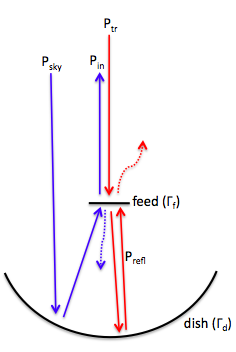
\includegraphics[totalheight=0.5\textheight]{plots/reflection_cartoon.png}
\caption{The blue solid lines represent an original sky signal entering the feed. A small percentage of it (dashed blue) is reflected off the dish, and it is these reflections that we are concerned about. In our measurements however, the reflections measured contain most of the original pulse signal (solid red), so it is crucial to adjust for this difference in our analysis.}
\label{fig:cartoon}
\end{figure}



\section{Reflection of the sky signal during observation:}

\begin{figure}
\centering
\includegraphics[totalheight=0.5\textheight]{schematic.pdf}
\caption{Schematic diagram showing reflection between the dish and the feed when sky signal is incident on it. }
\label{reflection_schematic}
\end{figure}
Figure \ref{reflection_schematic} shows the schematic of the sky signal propagation path during an observation. The plane wavefront from the sky is incident on the parabolic dish and focussed at the feed. A part of this power is reflected off the feed, incidents back on the dish and comes back to the feed after further reflection from the dish. We consider one reflection off the feed and subsequent reflection off the dish as one reflection. If the incident power is $P_{sky}$, feed power reflection coefficient is $\Gamma_{a}$ and the dish reflection coefficient is $\Gamma_{d}$ then the net power entering the feed after $n$ reflection of the feed and the dish,  

\begin{equation}
P_{in} =  P_{sky}(1-\Gamma_{a})\Gamma_{d} [1+ \Gamma_{a}\Gamma_{d} e^{i\phi}+ (\Gamma_{a}\Gamma_{d})^2e^{i2\phi}+ ....+ (\Gamma_{d}\Gamma_{n})^{n}e^{in\phi}]
\end{equation}

where, $\phi = ({2\pi \over c})f 2l$ is the propagation delay of the a frequency $f$ due to reflection over the focal distance $l$. 
Therefore, 
\begin{eqnarray}
{P_{in} \over P_{sky} } & = & (1-\Gamma_{a})\Gamma_{d} [1+ \Gamma_{a}\Gamma_{d} e^{i\phi}+ (\Gamma_{a}\Gamma_{d})^2e^{i2\phi}+ ....+ (\Gamma_{d}\Gamma_{n})^{n}e^{in\phi}] \nonumber\\
      & = & (1-\Gamma_{a})\Gamma_{d} {1-(\Gamma_{d}\Gamma_{a})^{n} \over 1-\Gamma_{d} \Gamma_{a} } 
\end{eqnarray}


Therefore, the input signal would have ripples of various frequencies over its passband which would manifest itself as a non-zero signal at various delays in the delay domain. We aim to measure the relative signal strength at various delays, referred to as "delay spectrum" hereafter, to estimate various level of reflections in between the feed and the dish apex.\\
 
 Delay spectrum measurement of the system is accomplished by measuring the return loss of the feed while keeping it at the focal point of the dish. A broadband signal $P_{tr}$ is sent to the feed antenna via a 75m long cable by the measuring instrument which is a vector network analyser (VNA). When the signal is incident on the feed, $\Gamma_{a}$ part of the incident power is reflected back to the measuring device and $(1-\Gamma_{a})$ part is radiated by the feed. The signal radiated by the feed illuminates the dish and is radiated out to the space. However, the signal incident at the dish apex is reflected by the dish and returns to the feed. This incident signal is now reflected back and forth in between the feed and the dish much like the sky signal reflection discussed previously. Hence, if $P_{r}$ is the power incident back on the feed for the first time then the reflected power $P_{ref}$ back into the measuring instrument would be, 

\begin{equation}
P_{ref} =  P_{r}(1-\Gamma_{a}) [1+ \Gamma_{a}\Gamma_{d} e^{i\phi}+ (\Gamma_{a}\Gamma_{d})^2e^{i2\phi}+ ....+ (\Gamma_{d}\Gamma_{n})^{n}e^{in\phi}]
\end{equation}
 
Once again we consider one reflection from the feed and subsequent reflection from the dish as one reflection. 

Now, $P_{r}$ is the power incident back on the feed which is the feed radiated power reflected off the dish.  
\begin{equation}
P_{r}= \Gamma_{d}(1-\Gamma_a) P_{tr}
\end{equation}
Also, the first reflection of the power sent by the measuring device occurs at the antenna end. Hence the total reflected power $P_{ret}$, returned to the measuring device would be, 


\begin{eqnarray}
P_{ret} & = & \Gamma_{a}P_{tr} \nonumber\\ 
 & & +  \Gamma_{d}(1-\Gamma_a) P_{tr}(1-\Gamma_{a}) [1+ \Gamma_{a}\Gamma_{d} e^{i\phi}+  ....+ (\Gamma_{d}\Gamma_{n})^{n}e^{in\phi}]\nonumber\\
 \end{eqnarray}
 Simplifying, 
 \begin{eqnarray}
 {P_{ret} \over P_{tr} } & = & \Gamma_{a}
  +  \Gamma_{d}(1-\Gamma_a)^{2}  {1-(\Gamma_{d}\Gamma_{a})^{n} \over 1-\Gamma_{d} \Gamma_{a} } \nonumber\\
\end{eqnarray}

 
The VNA measures the magnitude and phase of the quantity ${P_{ret}\over P_{tr}}$ as a function of frequencies which is plotted in figure \ref{fig:freq}. Since in this measurement set up, the first reflection occurs at the antenna terminal which is represented by $\Gamma_{a}$ in the above equation, $({P_{ret} \over P_{tr} }  - \Gamma_{a}) $ gives the estimate of the delay spectrum of the sky signal. In the delay domain, the relative signal strength at zero delay represents the factor$\Gamma_{a}$ while the signal strength at any other delay represents the any delayed signal that entered the feed after being reflected from the feed surroundings. 
 








\section{Methodology}

To measure the delays associated with reflections within the dish and feed, we
used the prototype HERA dish (Figure \ref{fig:heradish} built at the NRAO site in
Green Bank, WV. The dish is a 14-m parabolic reflector structurally supported
with 3 telephone poles. The reflective material is made up of wire mesh that
is attached to PVC pipes that form the parabolic shape. With the current
prototype, the feed is a PAPER dipole encased in a cylindrical cage encompassing
the backplane. The PAPER feed and the backplane (which prevents feed-to-feed
interaction between neighboring dishes) is raised and lowered by a three-pulley
system. The focal height of the dish is 4.5m ($\sim{14.76}$ft). Feed heights quoted in our measurements represent the distance from the balun to the top of the central concrete hub. Note, however, that the actual focal height of the dish represents the distance from the backplane of the feed to the dish's wire mesh, which intersects the concrete hub between the ground and the top of the hub. 
%XXX get discrepancy distance from DaveD.

The following reflectometry measurements were taken on July 20-23, 2015 using a
FieldFox unit in Network Analyzer mode. A pulse is generated in the FieldFox
and sent through a 75ft $50\Omega$ cable that connects to the feed with a 4:1
passive balun. The return loss as a function of frequency is saved. Both
the amplitude of the power and phase information are saved. Our
measurements are taken for a frequency bandwidth of 50 to 500MHz. 

Measurements are transformed into the delay domain during post-processing so that window functions
can be used in the Fourier transform. Without a window function, taking the Fourier transform of a finite data series (such as the return loss over a finite bandwidth), which can be interpreted as a square window function, is equivalent to convolving the Fourier transformed data with a $sinc$ function. This results in excess power at high delays due to the sidelobes in the $sinc$ function. Consequently, we have chosen to use a Blackman-Harris window function when moving into the delay domain. The effectiveness of this window function compared to a square window function is illustrated in Figure \ref{fig:window}.

\begin{figure}
\centering
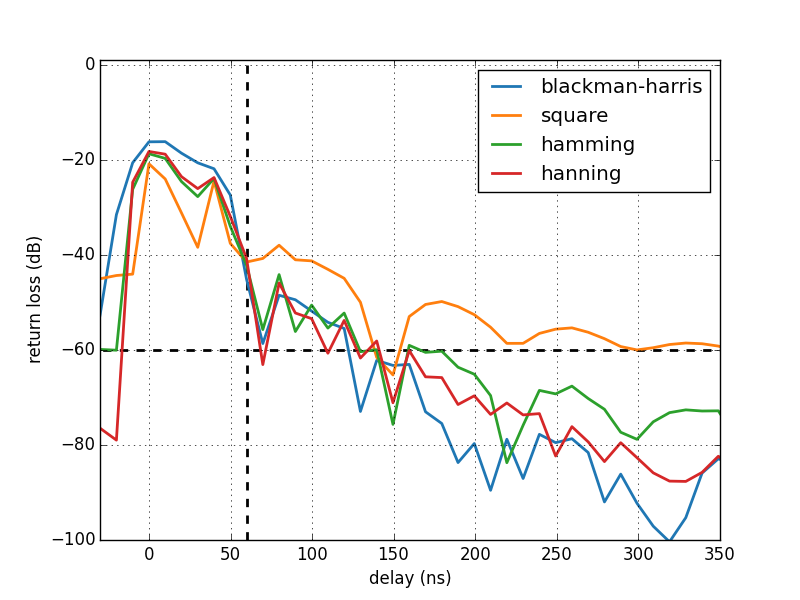
\includegraphics[totalheight=0.5\textheight]{plots/bh_vs_sq.png}
\caption{Delay plot produced using a Blackman-Harris window function vs. a square window function for the PAPER bandwidth.}
\label{fig:window}
\end{figure}

As mentioned in Section \ref{sec:theory}, there is a mis-match in amplitude between the reflections that we measure (originating from the FieldFox pulse) and reflections produced by sky signal. To compensate, we multiply our entire windowed delay spectrum by the DC component of the un-windowed delay spectrum.

\begin{figure}
\centering
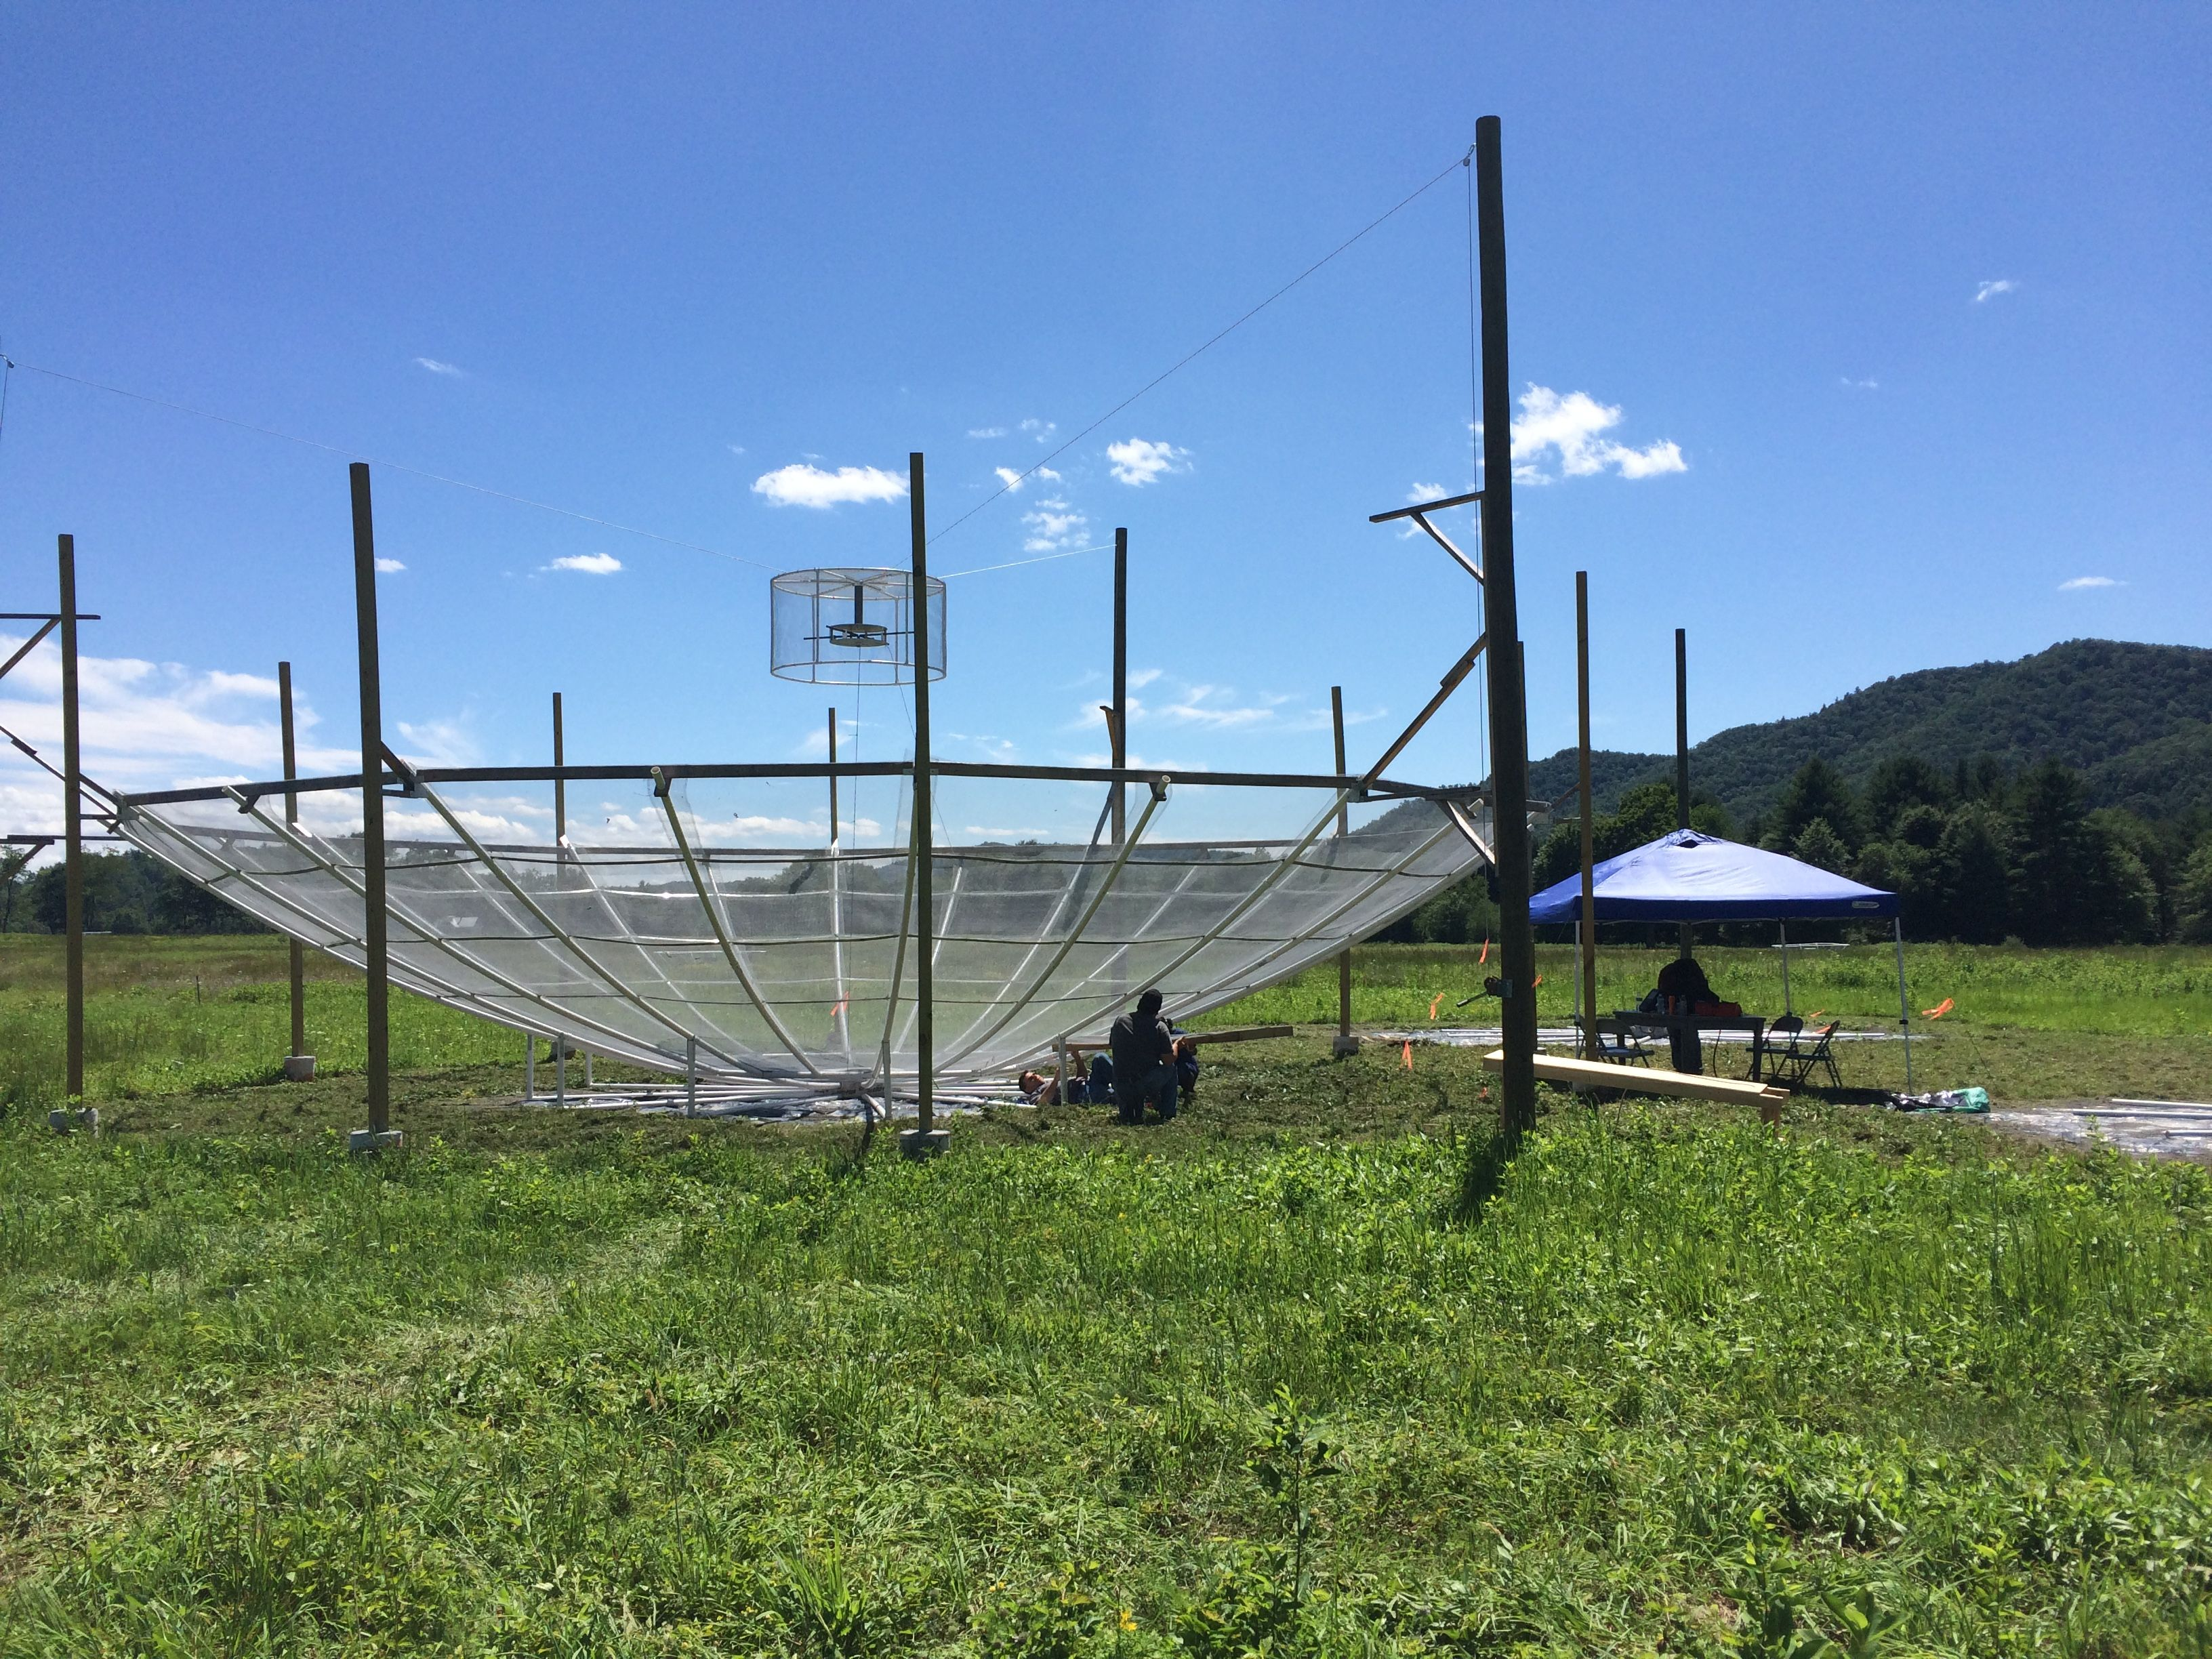
\includegraphics[trim={2cm 20cm 30cm 15cm},clip, totalheight=0.45\textheight]{plots/heradish.jpg}
\caption{HERA dish and feed at the Green Bank NRAO site.}
\label{fig:heradish}
\end{figure}

\section{Results}

Figure \ref{fig:freq} shows the return loss for a frequency bandwidth of 50 to 500MHz. This measurement was taken with the feed suspended at 12ft (distance between the balun and top of the central concrete hub). Because the return loss is the ratio of the power received to the power transmitted, higher reflections can clearly be seen outside of the PAPER bandwidth. This is not surprising, since the feed is tuned specifically for PAPER. The return loss minima are locations where our feed is well-matched to free space.

\begin{figure}
\centering
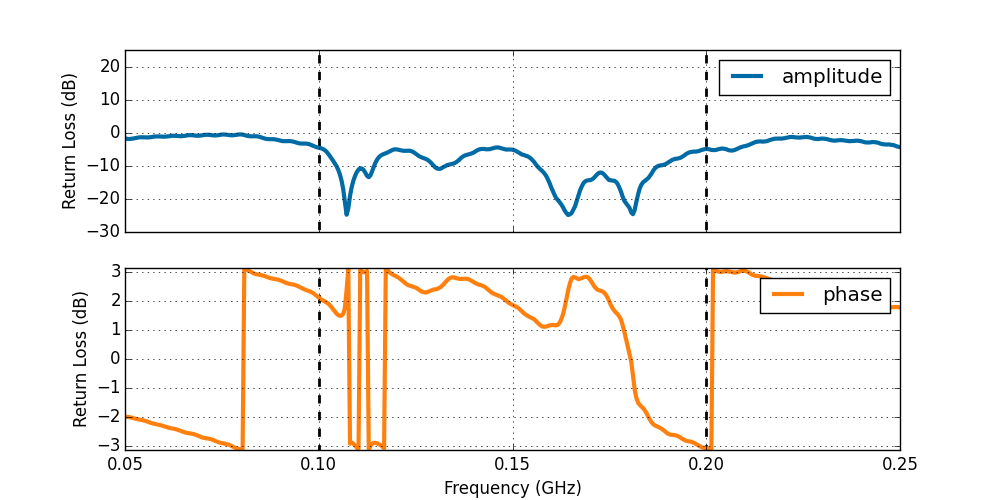
\includegraphics[totalheight=0.4\textheight]{plots/frequency_amp_phase.png}
\caption{Amplitude and phase of the measured return loss.}
\label{fig:freq}
\end{figure}

In Figure \ref{fig:3bands}, the return loss is plotted versus delay for three chosen bandwidths: the HERA bandwidth, the PAPER bandwidth, and a typical power spectra bandwidth when using a Blackman-Harris window function. It is again shown that the reflections are minimized for the PAPER bandwidth. 

\begin{figure}
\centering
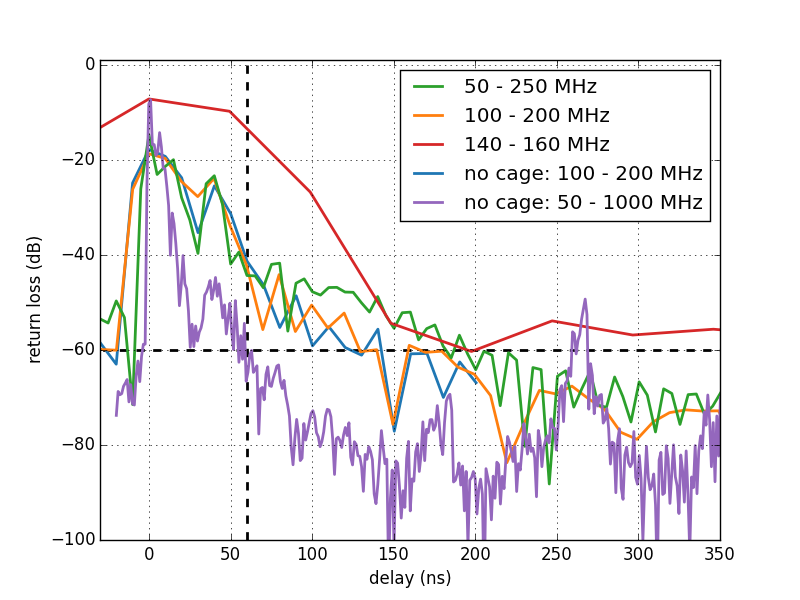
\includegraphics[totalheight=0.5\textheight]{plots/delay3_window.png}
\caption{Delay plots produced using a Blackman-Harris window function for 3 different frequency bandwidths: 50MHz-250MHz (``hera"), 100MHz-200MHz (``paper"), and 140MHz-160MHz (``pspec"). The black dashed lines illustrate our ``60 by 60" specification.}
\label{fig:3bands}
\end{figure}

Figure \ref{fig:elevator} is again a delay plot of the return loss, but for four different feed suspension heights. We use the PAPER bandwidth and note that the measurements are near identical at low delays, implying that low delay reflections are caused primarily by reflections within the feed cage. However, at higher delays we notice discrepancies between the different heights.

\begin{figure}
\centering
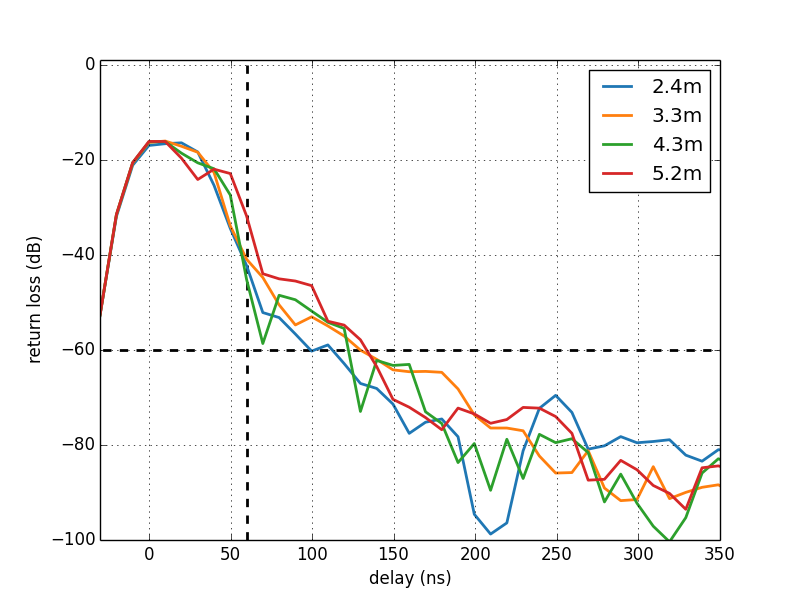
\includegraphics[totalheight=0.5\textheight]{plots/delay_heights_paper.png}
\caption{Delay plots produced using a Blackman-Harris window function for 4 different feed heights and the PAPER bandwidth. The black dashed lines illustrate our ``60 by 60" specification.}
\label{fig:elevator}
\end{figure}

Finally, Figure \ref{fig:outofthedish} presents measurements taken of the feed away from the dish. Echosorb is placed under the feed for some of the measurements, with the expectation that it will prevent any reflections off the ground. Measurements are also taken of the feed inside its metal cage in various configurations. 

\begin{figure}
\centering
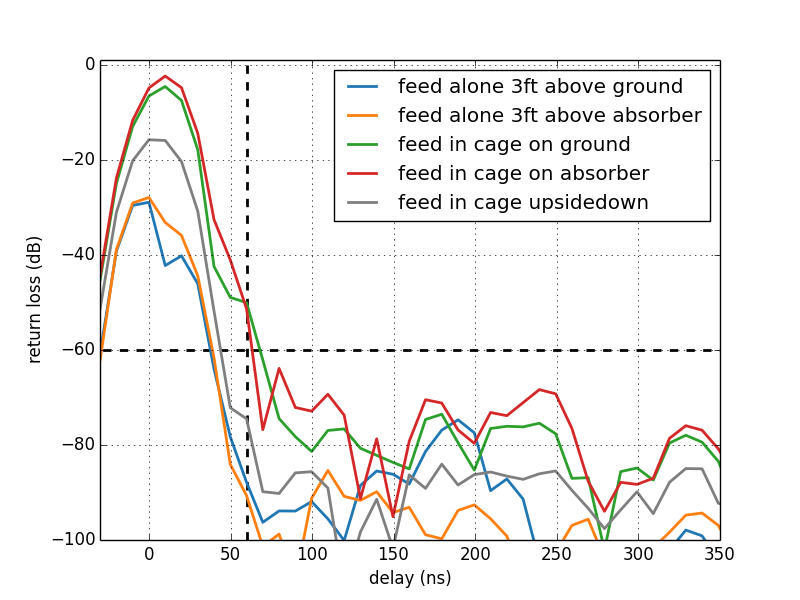
\includegraphics[totalheight=0.5\textheight]{plots/delay_feed.png}
\caption{Delay plots produced using a Blackman-Harris window function for different lone feed configurations and the PAPER bandwidth. The black dashed lines illustrate our ``60 by 60" specification.}
\label{fig:outofthedish}
\end{figure}


\section{Conclusion}


\end{document}
